\documentclass[12pt,a4paper]{article}
\usepackage[utf8]{inputenc}
\usepackage[spanish]{babel}
\usepackage{geometry}
\geometry{left=2.5cm,right=2.5cm,top=3cm,bottom=3cm}
\usepackage{graphicx}
\usepackage{hyperref}
\usepackage{fancyhdr}
\usepackage{titlesec}
\usepackage{xcolor}
\usepackage{listings}
\usepackage{enumitem}
\usepackage{amssymb}
\usepackage{float}

% Configuración de encabezados y pies de página
\pagestyle{fancy}
\fancyhf{}
\fancyhead[L]{Pontificia Universidad Católica del Ecuador}
\fancyhead[R]{Manual del Sistema}
\fancyfoot[C]{\thepage}

% Títulos bonitos
\titleformat{\section}
  {\normalfont\Large\bfseries\color{teal}}{\thesection}{1em}{}
\titleformat{\subsection}
  {\normalfont\large\bfseries\color{black}}{\thesubsection}{1em}{}

% Configuración listings para código
\lstset{
    backgroundcolor=\color{gray!10},
    frame=single,
    basicstyle=\ttfamily\footnotesize,
    breaklines=true,
    keywordstyle=\color{blue}\bfseries,
    commentstyle=\color{gray}\it,
    stringstyle=\color{orange},
    showstringspaces=false,
    numbers=left,
    numberstyle=\tiny,
    xleftmargin=1em,
    xrightmargin=1em,
    tabsize=4
}

\begin{document}

% Portada
\begin{titlepage}
\begin{flushright}   
 \vspace*{-2cm}
 
\includegraphics[height=2.5cm]{logo puce.png} 
\end{flushright}
 \centering
 \vspace*{1cm}
 {\Huge\bfseries Manual del Sistema\\[1.5ex] \textit{Mis Gastos}}\\[2cm]
 {\Large Pontificia Universidad Católica del Ecuador}\\[1cm]
 {\large Carrera: Tec Desarrollo De Software}\\[0.5cm]
 {\large Asignatura: Programación II}\\[0.5cm]
 {\large Profesor: Kevin Viteri}\\[1cm]
 {\large Elaborado por:}\\[0.3cm]
 {\bfseries Ariel Rosero y Ahinoa Andino}\\[2cm]
 {\large Quito, \today}
 \vfill
\end{titlepage}

\tableofcontents
\newpage

\section{Introducción}
El presente manual tiene como propósito guiar al usuario en la instalación, configuración, uso y comprobación del sistema \textbf{Mis Gastos}. Su objetivo principal es que cualquier persona que siga estos pasos logre implementar el sistema correctamente y pueda verificar su funcionamiento mediante evidencias visuales.

\section{Requerimientos previos}
Antes de comenzar, asegúrate de tener instalado en tu sistema lo siguiente:

\begin{itemize}
    \item \textbf{Python 3.9 o superior}
    \item \textbf{Pip} (gestor de paquetes de Python)
    \item \textbf{Git} (opcional, para clonar el repositorio)
    \item \textbf{Un editor de código} (recomendado: VS Code, PyCharm, Sublime Text)
    \item \textbf{Navegador web} (Chrome, Firefox, Edge, etc.)
\end{itemize}

\textbf{Nota:} Se recomienda el uso de un entorno virtual para evitar conflictos de dependencias.

\section{Instalación y configuración}

\subsection{1. Clonar el repositorio o descargar el código}

Puedes clonar el repositorio si está en GitHub, o simplemente crear una carpeta y copiar los archivos proporcionados en este manual.

\begin{lstlisting}[language=bash]
git clone https://github.com/tu_usuario/tu_repositorio.git
cd tu_repositorio
\end{lstlisting}

\subsection{2. Crear y activar entorno virtual}

\begin{lstlisting}[language=bash]
python -m venv .venv
# Activar en Windows:
.venv\Scripts\activate
# Activar en Mac/Linux:
source .venv/bin/activate
\end{lstlisting}

\subsection{3. Instalar Django}

\begin{lstlisting}[language=bash]
pip install django
\end{lstlisting}

\subsection{4. Estructura de carpetas del proyecto}

\begin{itemize}
    \item \textbf{mis-gastos/} (carpeta principal del proyecto)
    \item \textbf{gastos/} (app principal)
    \item \textbf{gastos/static/gastos/} (CSS, JS, imágenes)
    \item \textbf{gastos/templates/gastos/} (archivos HTML)
\end{itemize}

Coloca las imágenes, archivos CSS y JS en las rutas señaladas.


\section{Estructura de archivos y código fuente}

\subsection{1. models.py}

\begin{lstlisting}[language=Python]
from django.db import models

class Gasto(models.Model):
    descripcion = models.CharField(max_length=120)
    monto = models.DecimalField(max_digits=10, decimal_places=2)
    fecha = models.DateField(auto_now_add=True)
\end{lstlisting}

\subsection{2. views.py}

\begin{lstlisting}[language=Python]
from django.shortcuts import render, redirect
from .models import Gasto
from django.db.models import Sum

def landing(request):
    gastos_count = Gasto.objects.count()
    total_gastado = Gasto.objects.aggregate(total=Sum('monto'))['total'] or 0
    return render(request, 'gastos/landing.html', {
        'gastos_count': gastos_count,
        'total_gastado': f"{total_gastado:.2f}"
    })
\end{lstlisting}

\subsection{3. urls.py (de la app gastos)}

\begin{lstlisting}[language=Python]
from django.urls import path
from . import views

urlpatterns = [
    path('', views.landing, name='landing'),
    path('agregar/', views.formulario_gasto, name='formulario_gasto'),
    path('historial/', views.listado_gastos, name='listado_gastos'),
]
\end{lstlisting}

\subsection{4. urls.py (del proyecto principal)}

\begin{lstlisting}[language=Python]
from django.contrib import admin
from django.urls import path, include

urlpatterns = [
    path('admin/', admin.site.urls),
    path('', include('gastos.urls')),
]
\end{lstlisting}

\subsection{5. settings.py (fragmento para archivos estáticos)}

\begin{lstlisting}[language=Python]
STATIC_URL = '/static/'
\end{lstlisting}

\section{Archivos de plantilla (HTML)}

\subsection{landing.html}
\begin{lstlisting}[language=HTML]
<!-- Fragmento representativo de landing.html -->
<div class="hero-content">
    <h1>Controla tus gastos<br>y alcanza tus metas</h1>
    <p>Lleva un seguimiento claro y ágil de todos tus movimientos.</p>
    <a href="" class="btn-principal">Empieza ahora</a>
</div>
\end{lstlisting}

\subsection{formulario.html}
\begin{lstlisting}[language=HTML]
<!-- Fragmento representativo de formulario.html -->
<form id="gastoForm" action="" method="post" class="form-gasto">
    
    <div class="campo-form">
        <label for="descripcion">Descripción</label>
        <input type="text" name="descripcion" id="descripcion" required>
    </div>
    <div class="campo-form">
        <label for="monto">Monto gastado</label>
        <input type="number" step="0.01" name="monto" id="monto" required>
    </div>
    <div id="form-message"></div>
    <button type="submit" class="btn-principal">Agregar Gasto</button>
</form>
\end{lstlisting}

\subsection{listado.html}
\begin{lstlisting}[language=HTML]
<!-- Fragmento representativo de listado.html -->
<ul class="gastos-list">
    
        <li class="gasto-item">
            <span class="descripcion">{{ gasto.descripcion }}</span>
            <span class="monto">${{ gasto.monto }}</span>
        </li>
    
        <li class="gasto-vacio">No hay gastos registrados aún.</li>
    
</ul>
\end{lstlisting}

\section{CSS (style.css)}

\begin{lstlisting}[language=CSS]
/* Fragmento representativo de style.css */
body {
    background: #f4f7fb;
    font-family: 'Inter', Arial, sans-serif;
    color: #253245;
}

.btn-principal {
    background: linear-gradient(90deg, #1abc9c 0%, #19857b 100%);
    color: #fff;
    border-radius: 28px;
    font-size: 1.25rem;
    font-weight: 700;
    border: none;
}
\end{lstlisting}

\section{JavaScript (scripts.js)}

\begin{lstlisting}[language=JavaScript]
document.addEventListener('DOMContentLoaded', function () {
    // Validación y feedback en el formulario de gasto
    const form = document.getElementById('gastoForm');
    const msg = document.getElementById('form-message');
    if (form && msg) {
        form.addEventListener('submit', function (e) {
            const descripcion = form.descripcion.value.trim();
            const monto = parseFloat(form.monto.value);
            if (!descripcion || isNaN(monto) || monto <= 0) {
                e.preventDefault();
                msg.textContent = "Por favor escribe una descripción válida y un monto mayor a 0.";
                msg.style.color = "#d32f2f";
                return false;
            }
        });
    }
});
\end{lstlisting}

\section{Ejecución del proyecto}

\subsection{1. Migrar la base de datos}

Antes de utilizar la aplicación, es necesario preparar la base de datos para que Django cree las tablas necesarias según los modelos definidos en el proyecto. Para ello, debes ejecutar los siguientes comandos en la terminal:

\begin{lstlisting}[language=bash]
python manage.py makemigrations
python manage.py migrate
\end{lstlisting}

\textbf{¿Qué hacen estos comandos?}

\begin{itemize}
    \item \texttt{makemigrations}: Prepara archivos de migración que describen los cambios necesarios en la base de datos a partir de los modelos de Python.
    \item \texttt{migrate}: Aplica esos cambios, creando o actualizando las tablas en la base de datos real.
\end{itemize}

Es un paso fundamental para que la aplicación pueda guardar y mostrar información correctamente.

\subsection{2. Ejecutar el servidor}

\begin{lstlisting}[language=bash]
python manage.py runserver
\end{lstlisting}

Abre tu navegador y entra a: \url{http://127.0.0.1:8000/}

\section{Evidencias de funcionamiento}
\caption{Página principal o landing}
\begin{figure}[H]
    \centering
    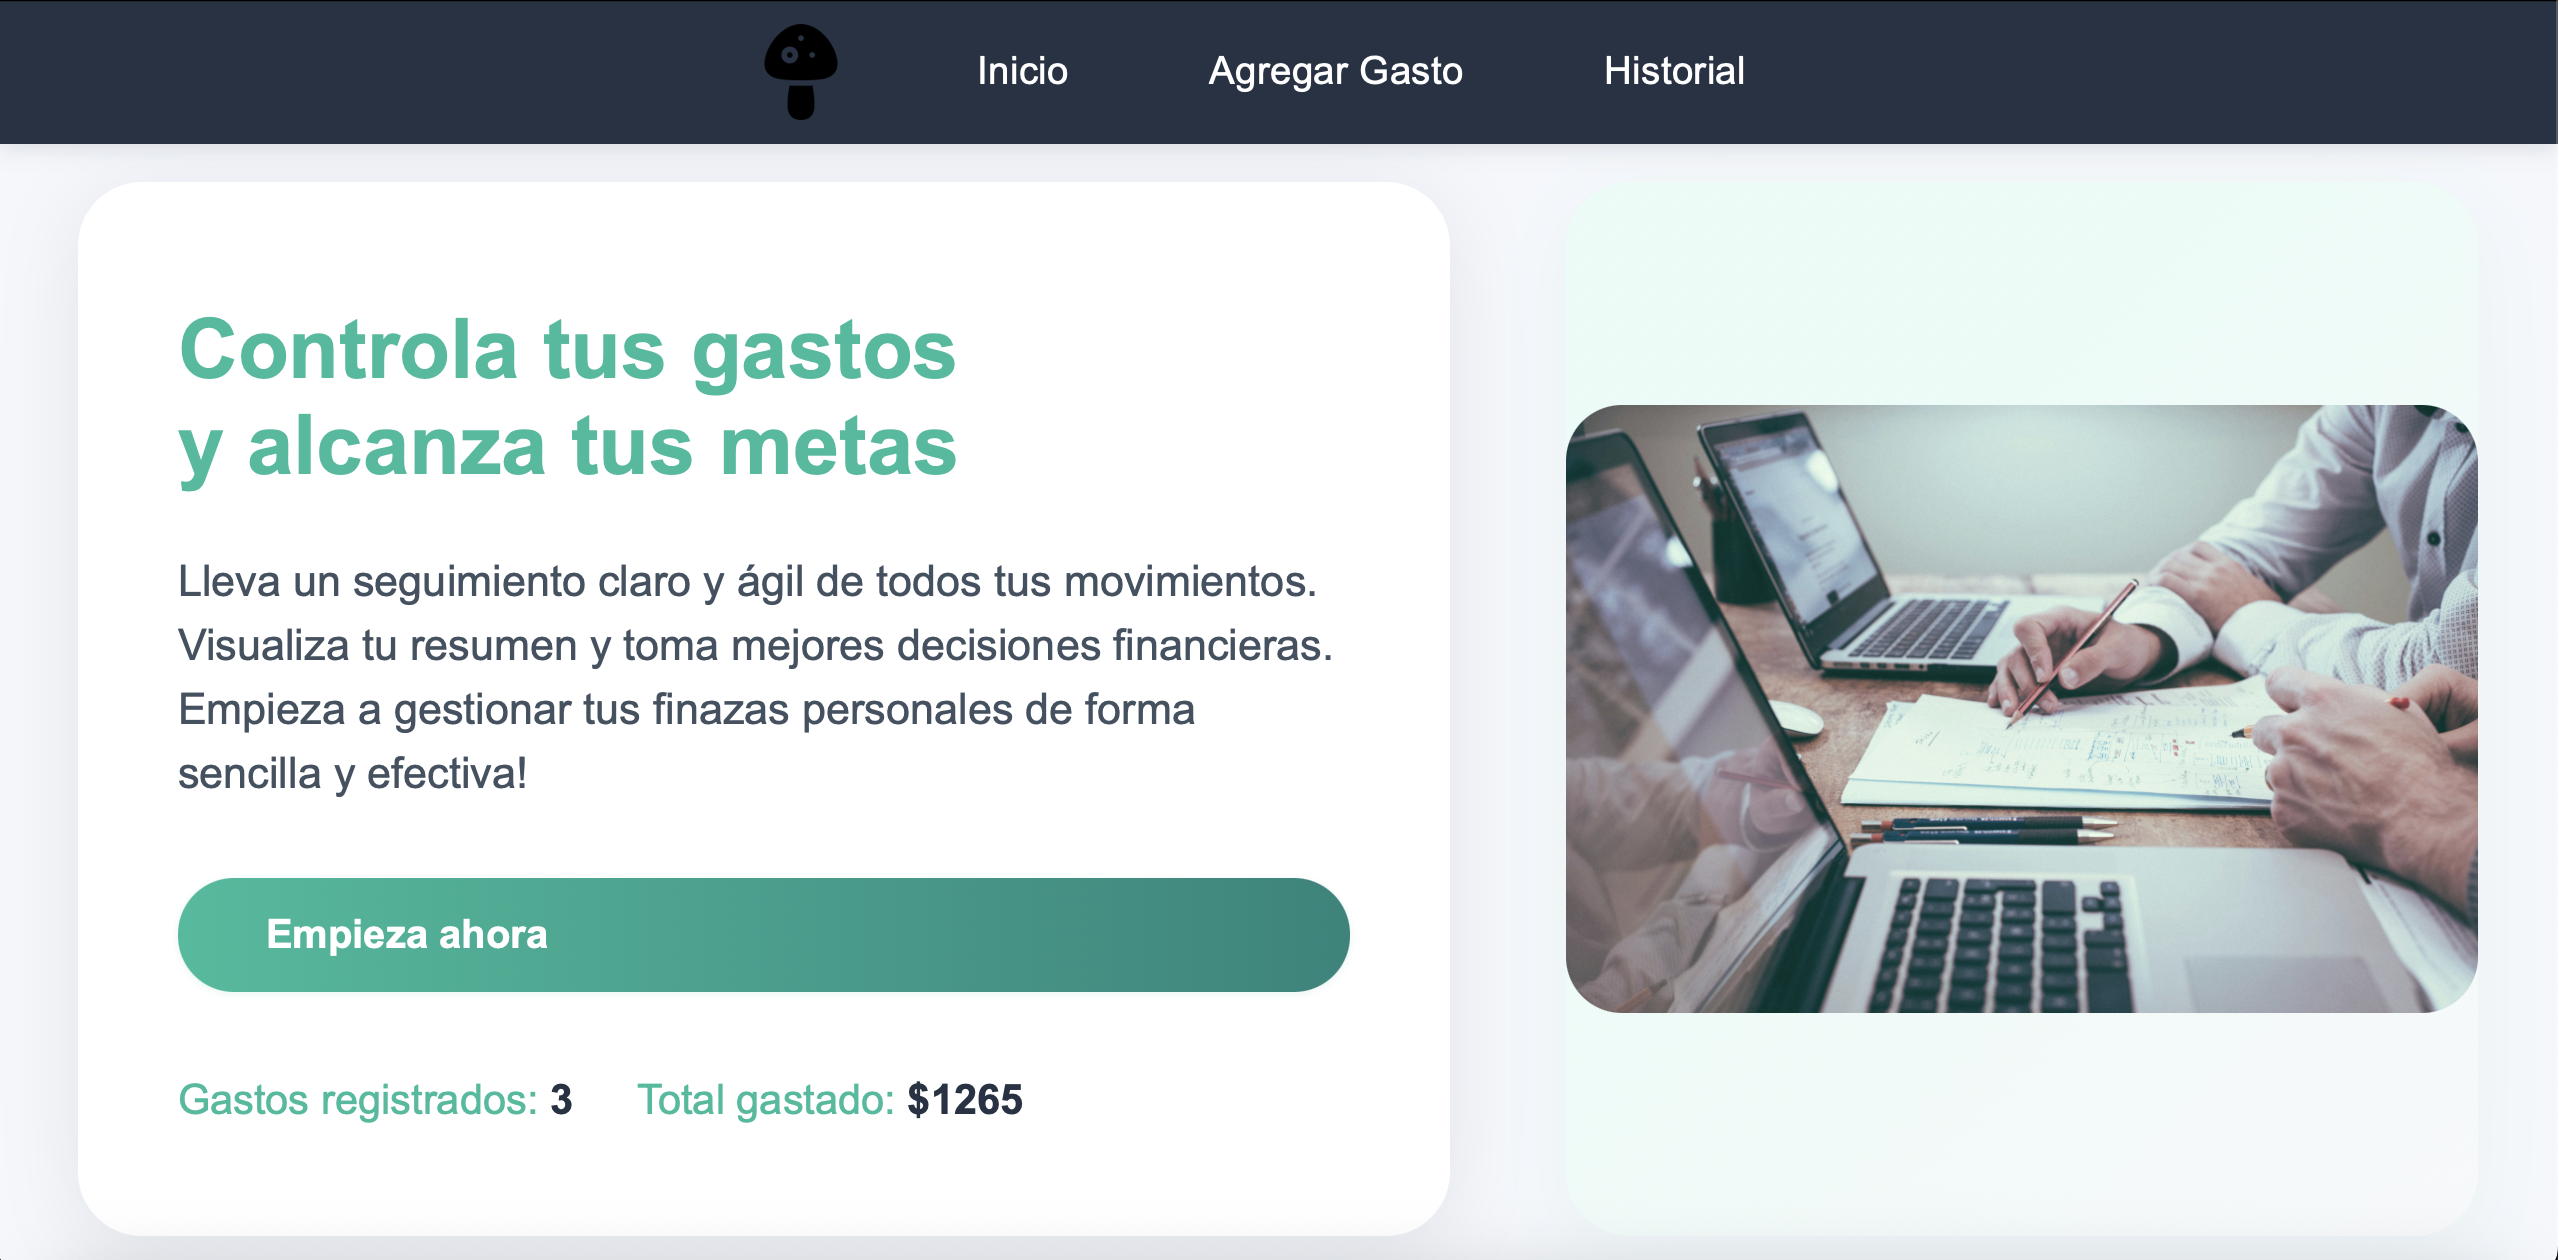
\includegraphics[width=0.85\textwidth]{Pagina Principal.png}
    \end{figure}
    
\caption{Formulario para agregar gastos}
\begin{figure}[H]
    \centering
    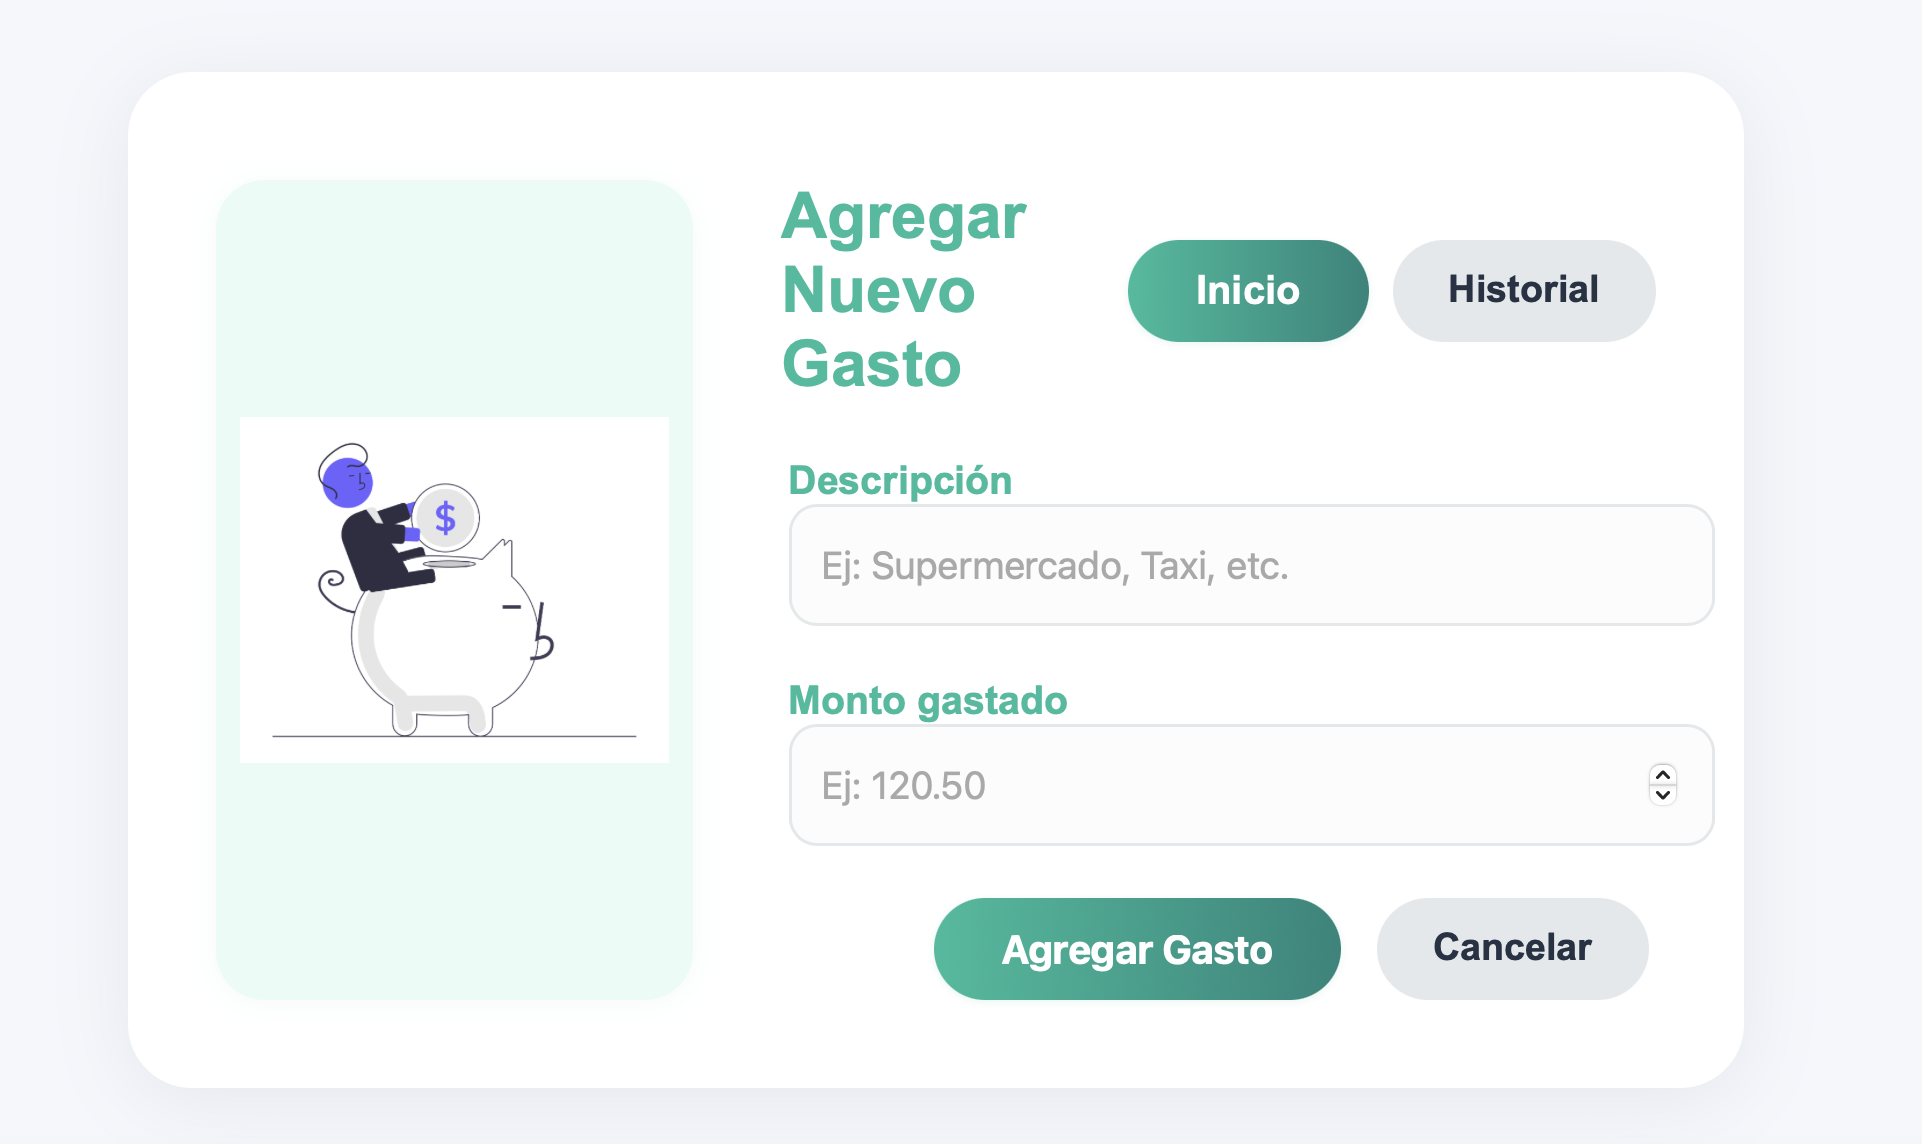
\includegraphics[width=0.85\textwidth]{Formulario.png}
    \end{figure}    

\caption{Historial de gastos}
\begin{figure}[H]
    \centering
    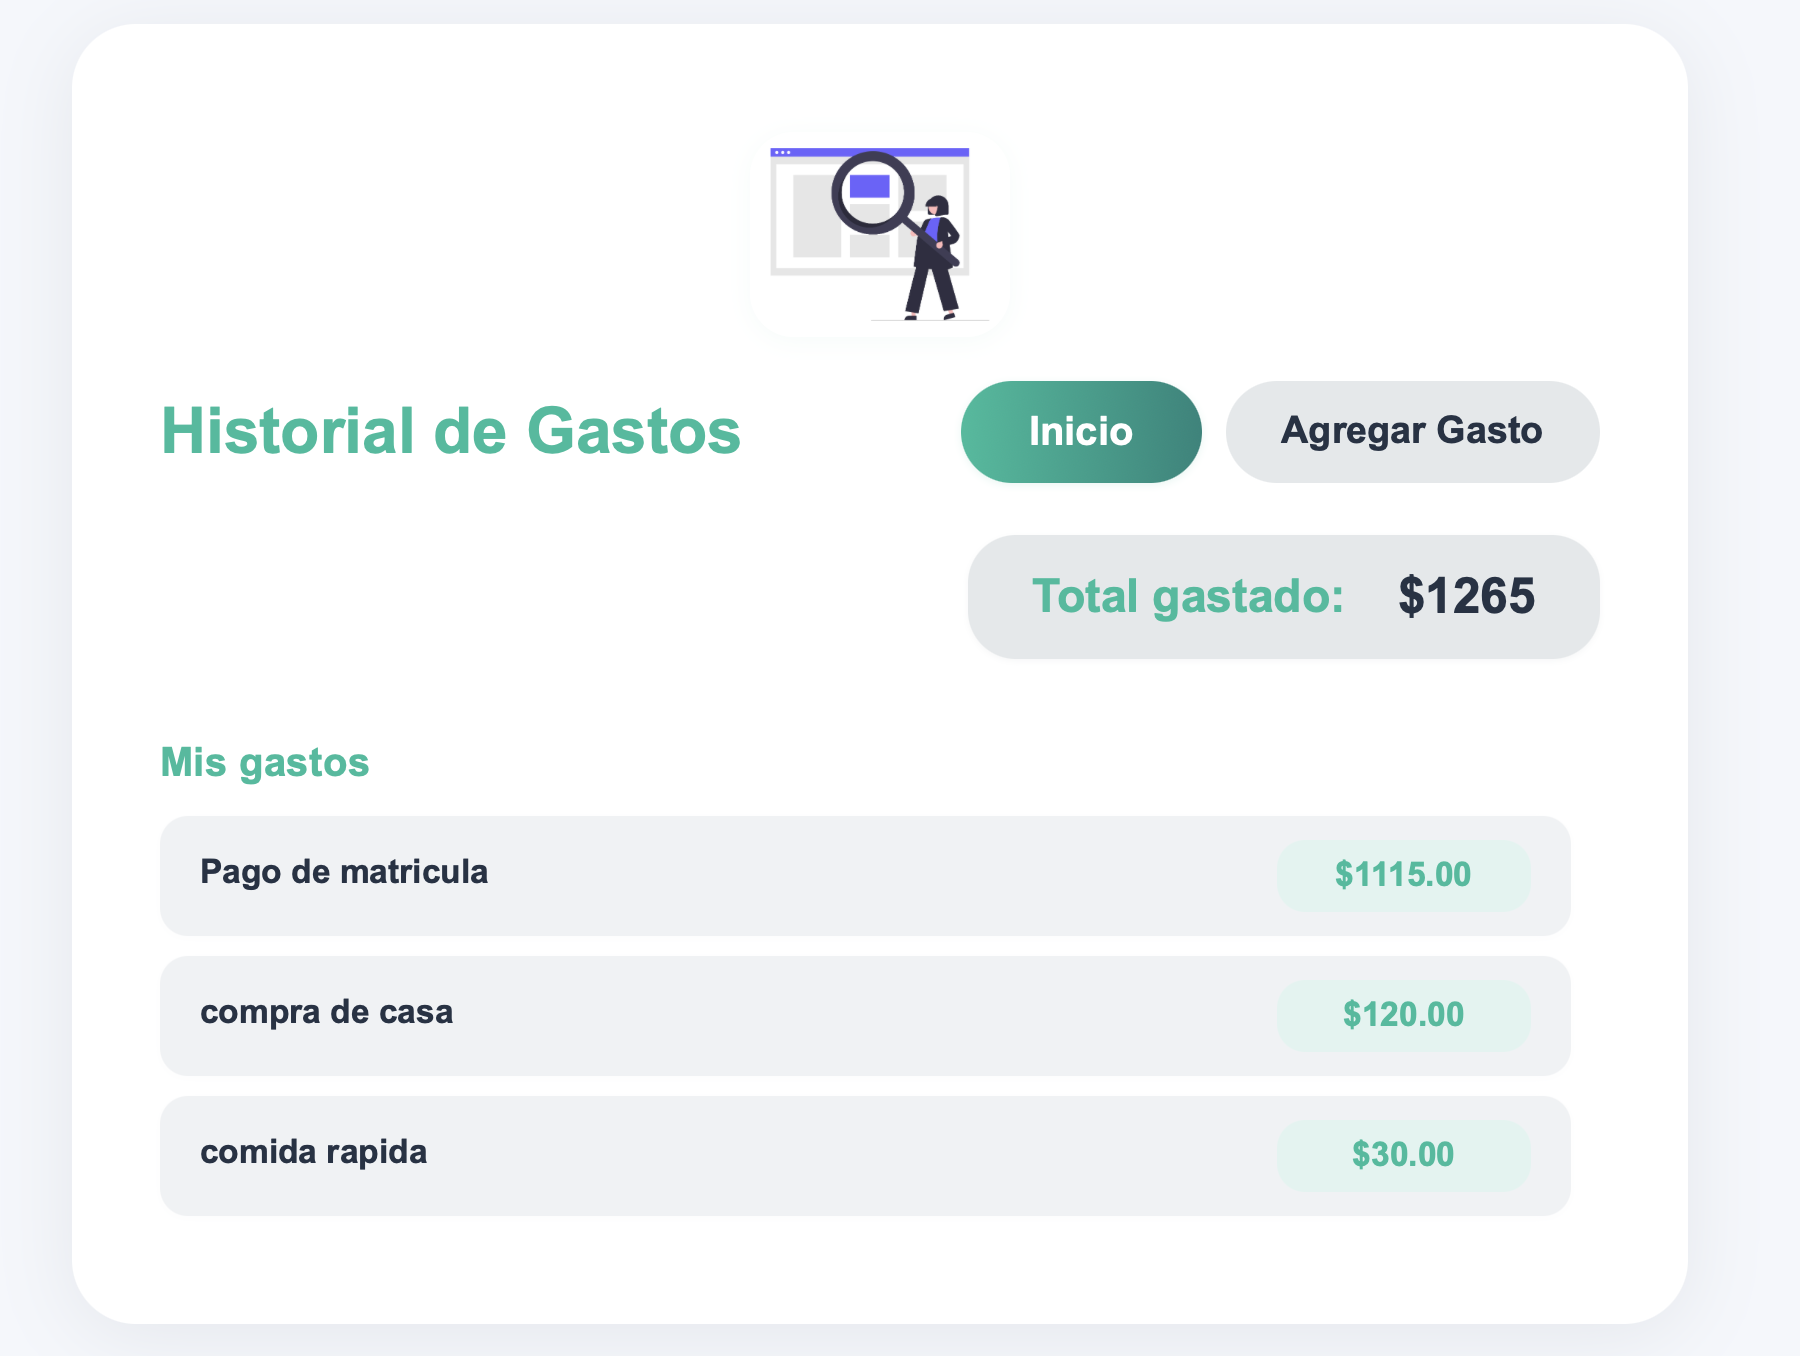
\includegraphics[width=0.75\textwidth]{Historial de gastos.png}
    \end{figure}
    
\section{Conclusión}

La finalidad de este manual es servir como una guía clara para la correcta instalación, configuración y uso de la aplicación “Mis Gastos”. Cualquier usuario podrá implementarlo y verificar su funcionamiento siguiendo los pasos aquí detallados.

\vfill
\begin{center}
    \textbf{ Fin del Manual }
\end{center}

\end{document}